%%
% The BIThesis Template for Bachelor Graduation Thesis
%
% 北京理工大学毕业设计(论文)第一章节 —— 使用 XeLaTeX 编译
%
% Copyright 2020 Spencer Woo
%
% This work may be distributed and/or modified under the
% conditions of the LaTeX Project Public License, either version 1.3
% of this license or (at your option) any later version.
% The latest version of this license is in
%   http://www.latex-project.org/lppl.txt
% and version 1.3 or later is part of all distributions of LaTeX
% version 2005/12/01 or later.
%
% This work has the LPPL maintenance status maintained'.
%
% The Current Maintainer of this work is Spencer Woo.
%
% 第二章节
\chapter{树状区块链}
本章中,介绍了树状区块链的应用场景,对其相关工作进行了简单调研,并详细描述其具体研究内容与原理,最终解决了树状区块链中合约部署与调用问题,完成了树状区块链的复现。
\section{背景介绍}
车联网是指车辆与车辆、行人、基础设施以及因特网的通讯的大型通信网络概念。在车联网中,主要有蜂窝移动网络和车载自组网两种不同的接入方式,车载自组网具备低成本、低时延以及地理位置天然联系的特性,是对蜂窝数据的重要补充,在道路安全等应用提供了重要支持\cite{klapez2020application}。

近年来,智能汽车的车辆数量变多,车辆与车辆、基础设施的交互也变得越来越多,势必导致数据安全、隐私、信任等相关安全性问题\cite{汤立波2019车联网产业融合发展趋势,VN2020}。区块链作为一种新型的互联网模式,具备去中心化、不可篡改、可追溯等特点,与车联网的联系愈发紧密,但实际应用上还是存在许多问题\cite{mollah2020blockchain}。其中主要包括两个问题,首先,区块链技术通常要求可靠的网络接入,存在网络覆盖以及基础设施成本问题 ,而车载自组网的接入方式由网络高动态性引发的网络不稳定对区块链的应用造成了极大的挑战。其次,车载自组网中的信息通常与地理信息天然绑定,而传统区块链并不具备此特性。因此,研究地理位置与区块链的融合就是为上述地理区域问题提供一种可能的解决方案。

\section{相关工作}
车联网与区块链的应用愈发紧密,然而,传统区块链的特点不能满足车载自组网的特性。一方面,传统区块链吞吐量较小、出块速度慢,需要改善它的结构来提升可扩展性;另一方面,传统区块链与真实世界的联系较弱,而车联网与地理信息有天然联系并且紧密相关,因此传统区块链结构不能很好适应车联网\cite{wagner2018cyber}。

就目前来说,一种主流的方案是将区块链的单链结构改良位多链结构\cite{global2020}。根据多链结构的构成方式的不同,可以将相关工作分为三类:并发多链\cite{parkmonoxide,zamani2018rapidchain,feng2019pruneable},层次多链 \cite{jo2018hybrid,liu2019mathsf,honar2021multi,qu2018blockchain,sharma2018blockchain,mbarek2019mbs,oktian2020hierarchical},智能合约多链\cite{sestrem2020cost}。并发多链存在多条子链,每条子链对应一个独立的功能模块,主链只负责维护多条子链的数据一致性;层次多链中,区块以层次化的结构组成区块链,各个层级具有上下从属关系;智能合约多链与并发多链结构类似,区别在于智能合约多链不修改区块链数据结构,通过智能合约维护多链数据一致性,存在多链数据同步的效率以及地理信息相关数据的存储以及检索的问题。而将地理位置融合进区块链的数据结构,实现层次化多链,这就是所谓的树状区块链。

\section{研究内容及原理}
由于全局同步与共识速度的限制,传统区块链不能很好的适应车载自组网的高动态性,极大的影响了区块链的效能,并且不能保证车辆与路侧节点的稳定连接,这将会极大影响到区块链共识机制的可用性。车载自组网与地理信息天然相联,并且车辆通常仅需要关注特定区域的信息,而传统区块链记录的交易信息不包含位置,无法根据地理区域查询交易,且传统区块链全局同步的设计会造成网络资源的大量浪费,并且传统区块链只能方便查询某个账户的交易、最新的交易、指定区块内包含的交易,无法高效的查询地理信息相关的数据。

树状区块链的研究就是为了解决上述问题,对区块链的结构进行修改与优化,使其更能适应车载自组网特性。树状区块链是一种基于位置的区块链,首先,根据GeoHash地理编码与地理区域层次关系建立树状结构的区块,同时研究树状结构地理信息相关数据查询速度的优化机制,从而提升区块链在车载自组网中的吞吐量以及与地理信息相关数据的检索速度。

GeoHash是一个能表示任意精度的高效地理编码系统,它使用二分法将指定区域分为网格,每个网格由唯一的编码表示,网络的大小对应的层次不同,编码越长对应的网格越小,层次越低。树状区块链使用GeoHash地理编码作为基本数据编码方式。建立 GeoHash 与区块以及交易的索引,从而依据GeoHash编码直接获取区域交易内容,同时,GeoHash编码可以通过前缀对区域信息进行绑定,因此通过GeoHash编码可以很自然地建立区域层次与子链的联系。

树状区块链主要包括三个部分的工作:更改区块数据结构、区块与节点的层次化分类以及区块的层次化组织。

\begin{enumerate}
 \item 区块链结构 \\
 如图\ref{树状区块链结构变化},树状区块链是基于以太坊的区块链数据结构进行修改的,在其基础上主要新增如下数据结构:\\
 \begin{figure}[!htb]
  \centering
  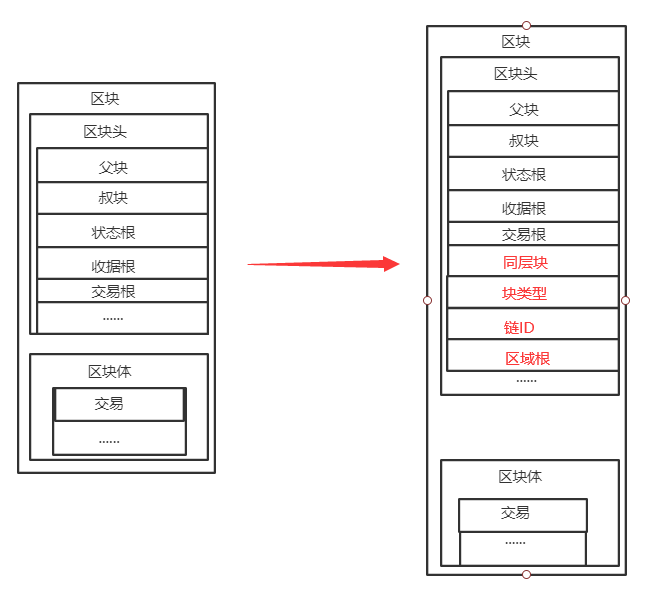
\includegraphics[width=5in]{images/1.png}
  \caption{树状区块链结构变化}\label{树状区块链结构变化} % label 用来在文中索引
\end{figure}

 \begin{enumerate}
  \item 同层块指针:记录与本区块同层次地理区域对应区块的哈希,与父块哈希一同构成树状区块链。
  \item 位置:使用指定长度的 Geohash 编码表示位置,分别在账户状态、交易数据中新增位置信息,增加账户、交易与物理世界的关联。
  \item 区域状态树:以Geohash作为索引构建字典树,存储区域内的四种信息:当前区域内的账户(Account)、交易(TXID)、收据(RPID)以及上层区域状态树根节点列表(URRList)记录所有上层区域状态树的根节点哈希,如图\ref{区域状态树}。
  
  \begin{figure}[!htb]
    \centering
    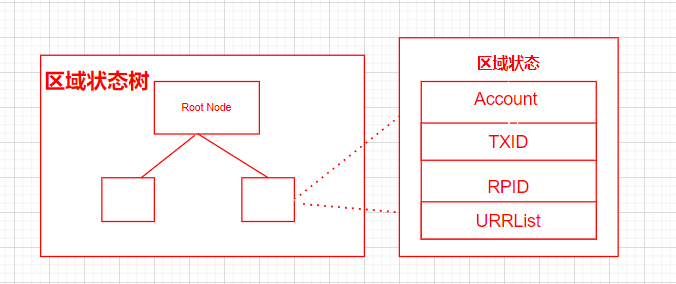
\includegraphics[width=5in]{images/14.png}
    \caption{区域状态树}\label{区域状态树} % label 用来在文中索引
  \end{figure}
  \item 账户位置树:在外部账户的账户状态中以发生交易时的,记录账户发生过的交易所在的区域。可以提供以下功能:根据位置区域,查询该区域内最新交易;查询某个账户在指定区域的交易以及历史交易发生的位置,如图\ref{账户状态树}。
  \begin{figure}[!htb]
    \centering
    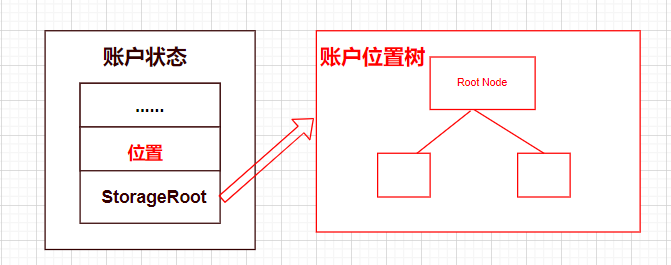
\includegraphics[width=5in]{images/15.png}
    \caption{账户状态树}\label{账户状态树} % label 用来在文中索引
  \end{figure}
 \end{enumerate}
 \item 区块与节点的层次化分类 \\ 为了将区块链划分为树状结构,首先将区块按其特征分为三种:
 \begin{enumerate}
  \item 创世块:区块链的初始区块。
  \item 分支块:根据 Geohash 编码以层次化结构一一对应创建分支区块作为对应区域内子链的头区块,只维护直接下层区域的索引信息,不记录交易信息。
  \item 普通块:地理区域的最小划分对应分支区块的子区块,记录在对应地理区域内发生的交易。
 \end{enumerate}
 其次,将网络节点按照其功能分为三种:
 \begin{enumerate}
  \item 全节点:维护全区块链完整区块数据和全局状态树,部分服务器为全节点。
  \item 区域节点:维护其所在区域内指定层次及以下的所有分支区块与普通区块。每个分支节点负责向上层节点更新汇总当前区域状态并同步所有上层区块链的区域状态树根节点列表。路侧节点与部分服务器为区域节点。
  \item 叶节点:维护所在区域内最下层分支区块以及普通区块。负责局部共识,以及在与区域节点有连接机会时上传缓存信息,并同步所有上层区块链的区域状态树根节点列表。车辆节点为叶节点。
 \end{enumerate}
 \item 区块的层次化组织 \par 
 在树状区块链设计中,只有普通区块会记录实际发生的交易,分支区块提供子区区块链头区块以及索引功能。每个地理区域都有对应一个分支区块和多个普通区块通过父块哈希指针组成的区块链,同层次不同区域多赢的分支区块之间通过同层块指针链接起来。分支区块的层次关系代表地理区域的包含关系,即上层分支区块对应的地理区域包含所有以该区块为父块的下层区块对应的地理区域。
\end{enumerate}

树状区块链与传统区块链相比,融合了地理位置,增加了区块链与真实世界的联系,设计了区块状态树和账户位置树提升与地理信息相关数据的检索速度。

\section{树状区块链的复现}
树状区块链是基于以太坊开发的。通过更改其以太坊底层区块链结构,增添区域状态树以及账户状态树,由go语言编译为新的geth客户端。本小节将对树状区块链所属geth客户端进行编译复现,并以此为基础建立一条基于树状区块链的私有链。

首先,下载源代码,配置go语言环境。从对应代码仓库将源码下载,使用go语言环境直接进行编译,生成最新版的树状区块链的geth客户端。为了方便后续使用,将该geth程序放入/usr/bin中。使用geth version确定geth能够正确使用。

然后,建立树状区块链私有链,创建创世块genesis.json文件,具体内容见附件C。
在同一文件夹下,初始化树状区块链私链:
\begin{center}
  \fbox{
    \parbox{130mm}{
      geth --identity "MyEth" --rpc --rpcaddr 127.0.0.1  --rpcport "8545" --rpccorsdomain "*" --datadir gethdata --port "30303" --nodiscover --rpcapi "eth,net,personal,web3" --networkid 91036 init genesisgtrie.json
    }
  }
\end{center}

在同一文件夹下,启动树状区块链:
\begin{center}
  \fbox{
    \parbox{130mm}{
      geth --identity "MyEth" --rpcaddr 127.0.0.1 --rpc --rpcport "8545" --rpccorsdomain "*" --datadir gethdata --port "30303" --nodiscover --rpcapi "eth,net,personal,web3" --networkid 91036 --allow-insecure-unlock --dev.period 1 console
    }
  }
\end{center}

创建新账户:
\begin{center}
  \fbox{
    \parbox{130mm}{
      personal.newAccount("123456")
    }
  }
\end{center}

输入测试数据,测试树状区块链功能函数:
\begin{center}
  \fbox{
    \parbox{130mm}{
      eth.getPosition(eth.accounts[0]) \# 查看账户位置 \\
      eth.getPosition(eth.accounts[0],1) \# 查询block=1时,accounts[0]的位置 \\
      eth.getStorageAt(eth.accounts[0],2)\# 查询在txtime=2时,accounts[0]的位置 \\
      eth.getAccountByRegion("wx111111111111") \# 根据GeoHash查询账户 \\
      eth.getTxByRegion("wx111111111111")      \# 根据GeoHash查询Tx信息 \\
      eth.getRpByRegion("wx111111111111")      \# 根据GeoHash查询Region信息 
    }
  }
\end{center}

以上内容,如果全部正确运行下来,没有出现报错,则证明复现成功,且树状区块链增添的相关位置信息的功能能够正常运行,至此完成复现。

 \section{树状区块链的合约部署与调用}
  在进行树状区块链合约部署的时候遇到两个问题,首先,与传统区块链不同,部署合约需要添加position和txttime参数,其次,在进行合约调用的时候,合约中的get方法中参数不能为空。

  目前,本文已经解决树状区块链部署问题,下面对其流程进行阐述。
  
  首先,运行私链,然后解锁帐户,合约可以使用truffle工具进行编译,在生成的Build文件夹下找到对应的json文件,获取其中的abi以及bytecode,随即在客户端上运行如下命令:
  \begin{center}
    \fbox{
        \parbox{130mm}{
        abi = JSON.parse('') \\
        bytecode = ""\\
        QualContract = web3.eth.contract(abi);
      }
    }
\end{center}

使用如下命令对部署合约所需要使用的Gas进行评估:
\begin{center}
  \fbox{
      web3.eth.estimateGas({data: bytecode})
  }
\end{center} 

如果在部署时合约对应部分,如果不添加position和txttime参数,树状区块链的私有链将会直接崩溃,所以在部署智能合约时需要增添对应参数,完成合约部署:
\begin{center}
  \fbox{
    \parbox{130mm}{
      Qual = QualContract.new(\{ \\
      from: web3.eth.accounts[0], \\
      data: bytecode, \\
      gas: '800000',\\
      position:"w25111111111113",\\
      txtime:277001\\
 \},function (e, contract)\{\\
      console.log(e, contract);\\
      if(!e)\{\\
          if(!contract.address) \{\\
              console.log("Contract transaction send: TransactionHash: " \par  + contract.transactionHash + " waiting to be mined...");\\
          \} \\else \{\\
              console.log("Contract mined! Address: " + contract.address);\\
              console.log(contract);\\
          \}
      \}
  \});
    }
  }
\end{center}

调用合约,合约调用中send方法也需要增添position和txttime参数,否则树状区块链也会崩溃,调用实例如下:
\begin{center}
  \fbox{
    \parbox{130mm}{
    trafficContract.methods.setSlingePos(userId, locTime[index], latOri, lonOri, latFix, lonFix).send(
    \{from: trafficContractAccount, gas: 500000,position:"w25111111111113",txttime:100\});
    }
  }
\end{center}

由于之前的树状区块链区块中,get方法中参数不能为空,为此,在树状区块链底层代码中get方式处增添缺省值,完成了对此问题的解决。

 \section{小结}
 本章中,首先,介绍了树状区块链的研究内容与原理,树状区块链对区块数据结构、区块与节点的层次化分类以及区块的层次化组织进行了研究,根据GeoHash地图编码与地理区域层次关系建立树状结构的区块,最终达到提升区块链在车载自组网中的应用范围。其次,根据前人相关工作完成了对树状区块链的复现,并解决了智能合约部署与调用的问题,使得树状区块链功能更加完整。